\documentclass[UTF8]{EPURapport}
%\usepackage{listings}

%\renewcommand{\lstlistlistingname}{Liste des codes}
%\renewcommand{\lstlistingname}{Code}

%\addextratables{%
%	\lstlistoflistings
%}

%\swapAuthorsAndSupervisors

\thedocument{Rapport de projet}{Canne connectée pour aveugles}{}
\grade{Département Informatique\\ 5\ieme{} année\\ 2020-2021}
\authors{%
	\category{Auteurs}{%
		\name{Djawad M'DALLAH MARI} \mail{djawad.mdallah-mari@etu.univ-tours.fr}
	}
	\details{DII5 2020-2021}
}
\supervisors{%
	\category{Encadrants}{%
		\name{Gilles VENTURINI} \mail{gilles.venturini@etu.univ-tours.fr}
	}
	\details{Université François-Rabelais, Tours}
}
\abstracts{Rapport du projet canne connecée pour aveugles}
{}
{}
{}

\begin{document}

\chapter{Remerciements}

Premièrement, je voudrais adresser mes remerciements à mon encadrant de projet, \textbf{M. Gilles VENTURINI}, initiateur de ce projet. Ses conseils et recommandations m'ont permis de mener au mieux ce projet. En outre, je voudrais remercier l'ensemble de l'équipe pédagogique de \textbf{Polytech Tours}, pour leurs efforts et engagements durant ces périodes scolaires. Leurs efforts m'ont apporté connaissances et compétences indispensables que j'ai pu mettre en pratique durant la réalisation de ce projet. Je tiens également à remercier mes camarades pour leur soutien et leur collaboration durant ces années d'études. 

\chapter{Introduction}
Ce document est le rapport du projet intitulé "canne connectée pour aveugles" réalisé dans le cadre d'un projet de fin d'étude (PFE) à Polytech Tours. Elle vise à synthétiser le travail réalisé en montrant les différents aspects du projet tels que la gestion organisationnelle, technique et humaine.\\

Ce projet de fin d'étude est donc un projet qui vise à mettre en pratique les acquis de ces dernières années, en mettant en particulier un accent sur les capacités d'analyses et de réflexion ainsi que la rigueur des solutions proposées pour répondre aux problématiques.\\

Nous verrons donc dans ce document les problèmes posés, les enjeux associés et les réflexions menées pour aboutir à des solutions. Nous verrons dans un premier temps une présentation du projet ainsi que ces objectifs. Nous aborderons ensuite la stratégie d'approche servant d'axe principal pour mener ce projet. Après, nous verrons les méthodes et outils de gestion de projet qui ont été mis en place. Les choix et réalisations seront ensuite présentés suivi d'une prise de recul détaillant notamment les points critiques et les difficultés rencontrées lors du projet. Enfin, une conclusion sera faite apportant quelques remarques personnelles sur le projet.

\chapter{Présentation}

\section{Contexte}

Ce projet a été initié afin d'étudier les possibilités offertes par un smartphone pour pourvoir aider les malvoyants dans leur quotidien. En effet, il existe aujourd'hui plusieurs modèles de cannes connectées qui permettent d'aider les malvoyants à se déplacer. Ces cannes se basent sur différentes technologies (GPS, capteurs de mouvement, etc.) afin de renvoyer des informations utiles aux utilisateurs tels que la détection de chute ou encore la géolocalisation de l'individu.\\

Ce projet vise donc à enrichir ces informations transmis à l'utilisateur pour lui permettre de mieux percevoir leurs environnements. Pour cela, on souhaite donc explorer le potentiel des smartphones, ainsi que de l'intelligence artificielle (IA) afin de recueillir le maximum d'information sur un environnement donnée. Cela nous permettra de voir également les limites de l'intelligence artificielle employée dans ce cadre là.

\section{Objectifs}

L'objectif de ce PFE est de faire de la reconnaissance d'image à l'aide du smartphone. Plus précisément, faire de la reconnaissance d'objet en réalisant une application Android. Cette application devra permettre de reconnaître les objets du quotidien (bouteille, assiette, mug, etc.) ou d'autres objets sur un environnement plus large (poteau, trottoir, arbre, etc.).\\

L’application devra ensuite informer l’utilisateur de l’objet identifié. Cette information devra être indiquée à l’utilisateur d’une manière particulière, car l’application est destinée à des personnes malvoyantes. Pour cela, une étude des habitudes d'utilisation des personnes aveugles de leur smartphone sera nécessaire afin de déterminer le meilleur moyen de renvoyer ce type d'information.\\

Le périmètre de ce projet sera donc autour de cet objectif principal qui est donc de fournir un prototype d'une application Android renvoyant des informations utiles sur la scène qui entoure l'utilisateur. Par la suite, une extension du périmètre initial du projet pourra être envisagée afin d'intégrer ce système sur une canne pour aveugles. Cette intégration pourra se faire par l'ajout du smartphone directement sur la canne ou par la réalisation d'un boîtier avec des capteurs communiquant avec le smartphone.\\

Sur ce point, M.VENTURINI avait travaillé avec d'autres étudiants sur la faisabilité de ce projet sur un microcontrôleur et travail également avec des étudiants du département informatique (DI) sur l'enrichissement d'un réseau de neurones afin de pouvoir enregistrer et reconnaître des objets donnés.\\

Notre application sera donc un premier prototype qui nous permettra d'avoir un premier outil qu'on pourra présenter aux personnes malvoyantes afin d'avoir un retour précis sur leurs besoins. L’Institut d’éducation sensorielle pour sourds et aveugles IRECOV de Tours peut nous permettre d'entrer en contact avec des personnes aveugles afin de réaliser des tests.\\

\chapter{Motivation et stratégie d'approche}

\section{Motivations}

J'ai été particulièrement intéressé par ce projet, car c'était une occasion pour moi de découvrir le domaine de l'intelligence artificielle et des réseaux de neurones. En effet, durant mes années d'études, je n'ai pas eu l'occasion de suivre des cours là-dessus ni de travailler sur des projets mettant en œuvre ce type de technique. Ceci, malgré qu'on en entend de plus en plus dans différents domaines d'application. Il me semblait donc intéressant de saisir cette occasion afin de m'initier et comprendre quelques mécanismes sur son fonctionnement.\\

J'ai aussi été attiré par le fait que ce travail pourrait servir concrètement à des personnes réelles et n'est donc pas qu'un simple projet académique permettant de mettre en œuvre les acquis. Un réel besoin existe auprès des utilisateurs finaux, ce qui motive fortement à être engagé afin de faire aboutir ce projet.\\

Un autre point est que, malgré le fait que je n'ai pas eu l'occasion de suivre des cours sur de l'intelligence artificielle ou le fonctionnement des réseaux de neurones, j'ai déjà de l'expérience dans la réalisation d'application Android. En effet, j'ai pu réaliser une application Android durant mon stage de DUT, et ça m'a permis non seulement de renforcer mes compétences en Java, mais aussi de découvrir le monde du développement mobile. L'aspect technique de ce projet n'est donc pas un frein pour moi, mais plutôt elle me permettra de me baser sur mes acquis afin d'appréhender l'intelligence artificielle sereinement.\\

Ce projet est donc un challenge qui me permettra de consolider mes acquis et d'élargir mes compétences et connaissances sur d'autres facettes de l'informatique.

\section{Stratégie d'approche}

Les enjeux du projet de fin d'études n'étant pas tournés autour de la technique, j'ai préféré me concentrer sur d'autres points tout aussi important dans ce type de projet. En effet, pour qu'un projet soit réussi, il faut être capable de prendre du recul et gérer les autres aspects autour de la technique telle que \textbf{la gestion du projet} au sens organisationnel, \textbf{anticiper les risques} et \textbf{respecter les délais et le budget}. Une de mes stratégies fut donc la mise en place de planning afin d'organiser chaque phase du projet du début à la fin.\\

Il faut également \textbf{être à l'écoute du client}. C'est pourquoi mettre en place une bonne \textbf{communication avec le client} est essentiel, car cela permettra de bien comprendre le besoin et donc d'être capable de fournir des solutions adéquates. Cette communication régulière permet également de faire un point sur l'avancement du projet et de valider les fonctionnalités implémentées. C'est donc une des stratégies que j'ai pu mettre en place avec le client de manière hebdomadaire par appel ou par mail.\\

Un point important est aussi le fait de fournir un travail qui pourra être repris facilement à la fin du projet. L'importance apportée aux livrables sur le projet de cette année permet donc de fournir des documents qui réunissent tous les éléments nécessaires à \textbf{la reprise du projet}. Ce rapport sera donc accompagné du cahier de spécification, le cahier d'analyse, le manuel développeur, le manuel mainteneur, le manuel administrateur ainsi que le manuel utilisateur. Ces documents faciliteront donc la reprise du projet. J'ai également commenté les parties les plus importantes du code source du projet, mais aussi essayer de respecter les normes de codage et les bonnes pratiques. Tout ceci sur mon github \footnote{ Code source: \url{https://github.com/Djawad-mdallahmari/PFE-ObjectDetection} \\ Documentation: \url{https://github.com/Djawad-mdallahmari/PFE-Documentation}} avec l'historique depuis le début du projet afin de pouvoir revenir sur d'anciennes versions si besoin.

\chapter{Gestion du projet}

\section{Plannings}

Parmi les éléments qui m'ont aidé à gérer mon temps, il y a le planning prévisionnel que j'ai établi en début de projet. Ce planning m'a permis de définir clairement chaque phase du projet et de leur attribuer un temps limité. Ceci, m'a donc forcé à respecter les délais que je me suis attribués pour chaque phase ainsi que les jalons prévus par Polytech sur les différents livrables à rendre. \\

\begin{figure}[h!]
\centering
  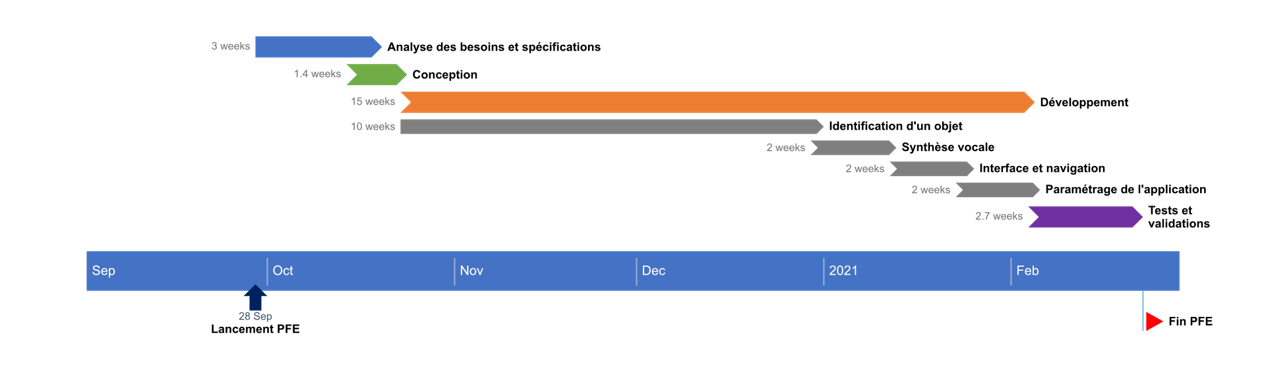
\includegraphics[width=\textwidth]{images/PlanningPrev.png}
  \caption{Planning prévisionnel}
  \label{fig:planningprev}
\end{figure}

Dans ce planning, j'ai décidé de rester assez général en indiquant seulement les grandes phases du projet sans détailler chaque tâche que j'allais faire. Ceci pour deux raisons : 

\begin{itemize}
  \item La première est le fait qu'à ce stade du projet, il est encore difficile d'imaginer chaque tâche et fonctionnalités que je serai amené à faire. En effet, au début du projet, il a fallu que j'étudie le besoin du client et ensuite faire une analyse de ces besoins afin de pouvoir proposer des solutions.
  \item La deuxième est que la définition de chaque tâche à faire en début du projet se traduira par une spécification figée qu'on ne pourra changer selon l'avancé du projet. Ce qui est une des inconvénients du cycle en V. J'ai donc voulu allier la méthode cycle en V en réutilisant ses différentes phases de projet tout en prenant quelques concepts du modèle agile en y introduisant une souplesse dans les spécifications ainsi que dans les tâches que je serai amené à réaliser.
\end{itemize}

En procédant ainsi, j'ai décidé de ne détailler que la phase de développement en y ajoutant les fonctionnalités que je devais implémenter et le temps que cela me prendrait (éléments en gris sur le planning).\\

Sur ce planning, j'ai décidé de ne pas représenter les tâches liées aux livrables. Ces tâches seront réalisées en parallèle des différentes phases du projet. Lors de la phase d'analyse et de spécification des besoins, j'ai rédigé en parallèle le cahier de spécification puis le cahier d'analyse. De même pour le rapport et les autres livrables qui seront rédigé vers la fin du projet. Cependant, il y a quelques écarts entre le planning prévisionnel et le planning réel. \\

\begin{figure}[h!]
\centering
  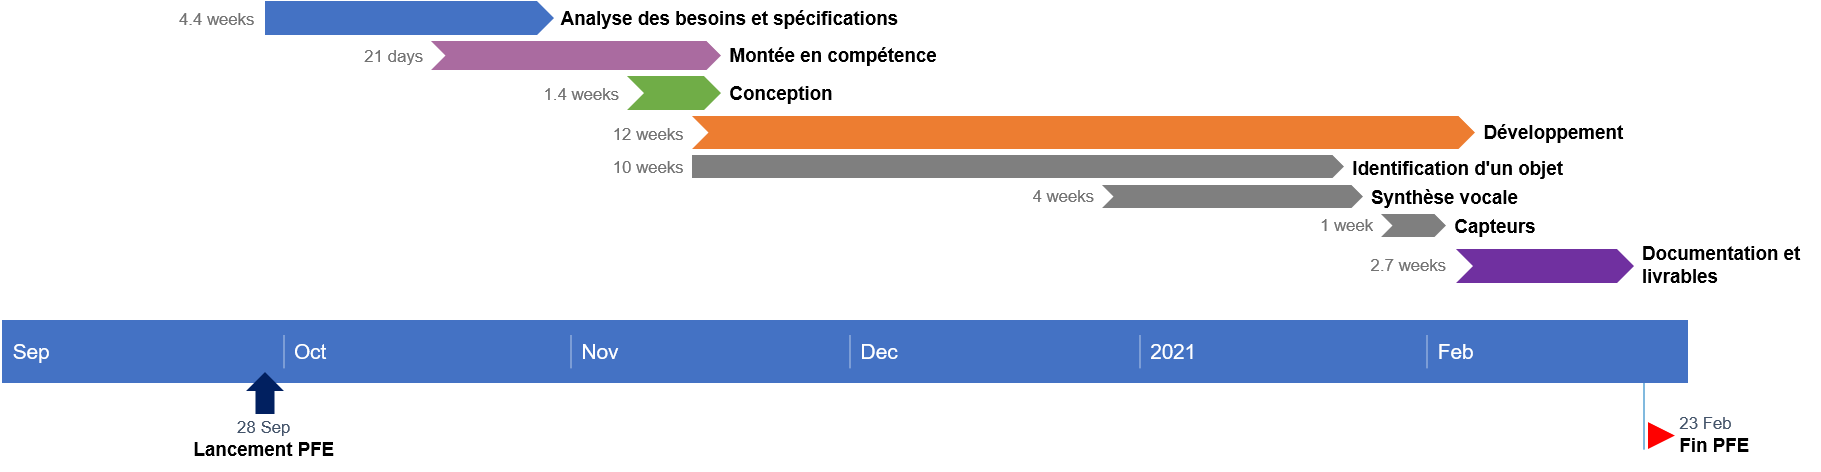
\includegraphics[width=\textwidth]{images/PlanningReel.png}
  \caption{Planning réel}
  \label{fig:planningreel}
\end{figure}

Dans le planning réel, la phase d'analyse a duré plus longtemps que prévu, car il a fallu que je monte en compétences afin de comprendre comment fonctionne l'intelligence artificielle, les technologies à utiliser pour l'implémenter, étudier les avantages et inconvénients de chacun etc. avant d'être capable de proposer une solution. J'ai donc empiéter sur la phase de développement, mais j'ai quand même commencé à regarder quelques codes très tôt et de les modifier afin de comprendre comment cela fonctionnait. \\

Ensuite, on remarque que certaines fonctionnalités comme la réalisation d'une interface de navigation a été omis. Ceci car en fonction de l'avancée du projet, on a remarqué cela n'était pas forcément utile puisque l'utilisateur n'a pas besoin d'accéder à d'autres menus. Dans notre application il y a qu'une barre qu'on peut faire apparaître afin de faire quelques réglages, mais l'utilisateur dans un premier temps n'aura pas besoin de régler ces paramètres-là pour utiliser l'application. \\

Cette modification est donc le résultat d'un suivi régulier qui a permis de déterminer ce qui est important de ce qui l'est moins. Nous avons donc utilisé ce temps afin de réfléchir à d'autres fonctionnalités qui pourraient nous être utiles comme la mise en place de différents capteurs. Dans l'optique de fournir à l'utilisateur un maximum d'informations sur un environnement donné, l'utilisation de ces informations venant des capteurs pourraient donc nous être plus utile que de réaliser une interface de navigation. 

\section{Gestion des tâches}

Pour la gestion des tâches de manière plus minutieuse, j'ai décidé de mettre en place un \textbf{Trello}. \\

\begin{figure}[h!]
\centering
  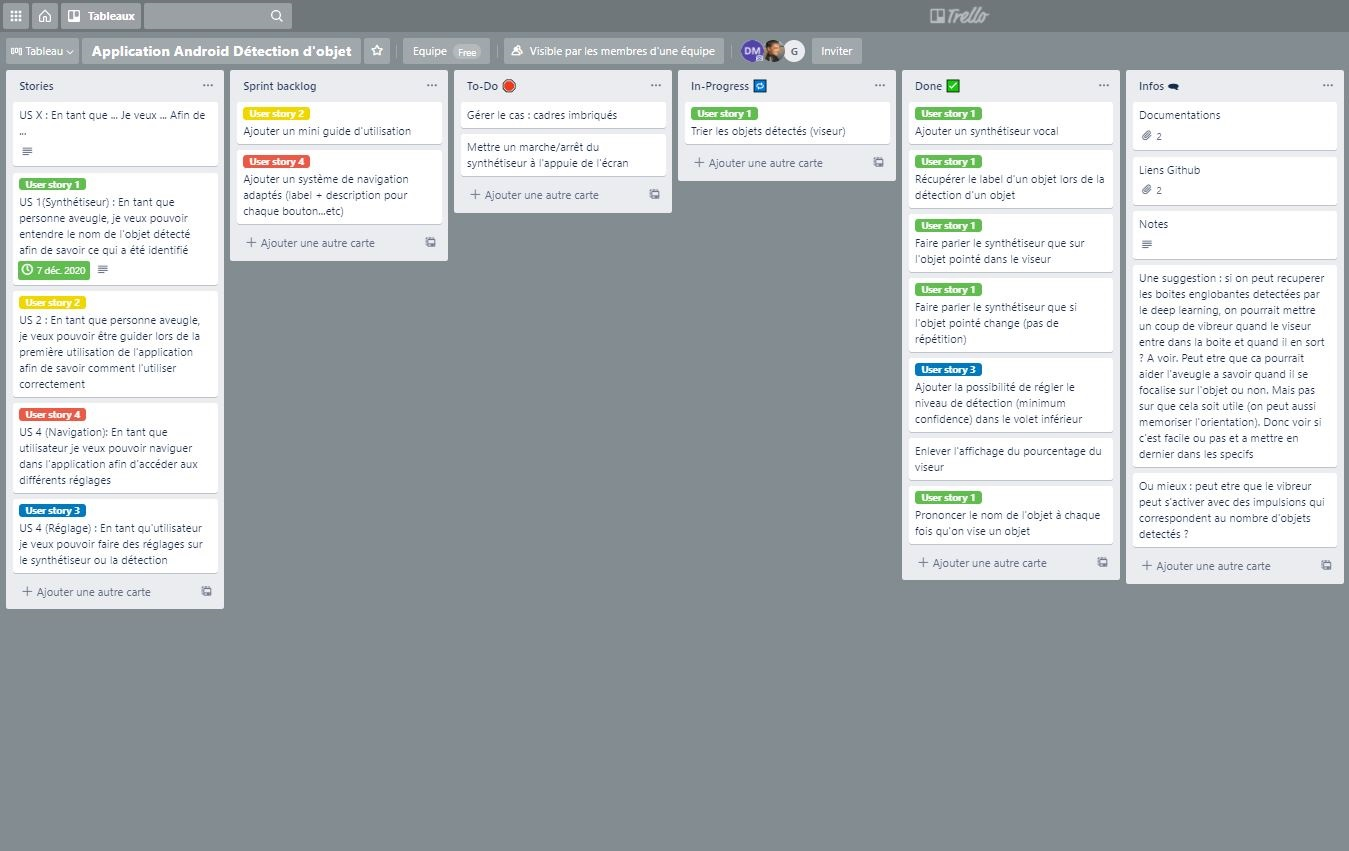
\includegraphics[width=\textwidth]{images/Trello1.JPG}
  \caption{Exemple état du Trello en phase développement}
  \label{fig:trello}
\end{figure}

Ce Trello m'a permis d'avoir une vue globale des tâches qui ont été faites et ceux qui restent à faire. J'ai décidé de l'organiser un peu à la manière des tableaux des méthodologies agiles puisque je venais le mettre à jour à la fin de nos réunions hebdomadaires avec le client. Cela permettait donc de valider ce qui avait été fait mais aussi de noter ce qui est à faire pour la prochaine réunion à la manière des sprints dans la méthodologie Scrum. De cette manière, je gardais donc une flexibilité sur les tâches à faire en fonction des retours du client tout en gardant un suivi sur la fonctionnalité auquel chaque tâche est liée. En effet, chaque tâche devait être liée à une fonctionnalité donnée qui répond à un besoin du client/utilisateur. C'est pour cela que j'ai décidé de décrire les fonctionnalités sous forme de User Story. En faisant ainsi, on comprend le besoin et le pourquoi de chaque tâche.\\

Cependant, un autre point que j'ai volontairement décidé de ne pas utiliser sur Trello est l'attribution d'une date butoir à chaque tâche ainsi que l'attribution d'une tâche à chacune des parties prenantes du projet. En effet, je partais de l'idée que les tâches les plus prioritaires sont ceux qui ont été discuté lors de la précédente réunion, je les passe donc dans la colonne "To Do" sans déterminer la date butoir ni prendre la peine de déterminer la personne qui devait la faire puisque ça allait forcément être moi-même. Ce point aurait été plus intéressant dans le cadre d'une équipe plus large avec plusieurs développeurs par exemple. \\

Je me suis donc inspiré de la méthode agile sur l'établissement de ce Trello sans pour autant être stricte sur les concepts de la méthode tel que l'établissement d'un backlog ou la production d'un MVP (Minimum Viable Product) à la fin de chaque sprint. 

\section{Versionning}

Afin d'avoir un suivi de chaque changement, que ce soit au niveau des documents ou au niveau du programme, j'ai utilisé \textbf{Git} dès le départ. Pour les documents, chaque version est écrite dans la première page du document (sauf la version finale). Cela permet donc de revenir à une ancienne version d'un document en ayant la date de la dernière modification.\\

Le git me permet également de stocker les différentes versions de tests de l'application (les .apk) que je déploie afin que le client puisse tester les nouvelles fonctionnalités implémentées. Ainsi, on garde un état de l'application après chaque déploiement. Si on souhaite déployer une nouvelle version de l'application sur le Google Play par exemple, ce système nous permet de revenir à la version précédente en cas de bug non identifié, mais remonté par les utilisateurs.\\

C'est donc un bon moyen de fournir l'ensemble du projet avec son historique afin que le projet soit repris facilement dans son entièreté \footnote{Attention, le github est sur mon compte étudiant et risque peut-être de disparaître lorsque mon compte étudiant ne sera plus valide. En cas de reprise du projet, il faudra veiller à cloner ces repository rapidement dès le départ.}.

\chapter{Choix et réalisations}

\section{Framework et modèle}

Pour répondre au \textbf{besoin d'identification d'un objet}, j'ai choisi d'utiliser la librairie \textbf{TensorFlow Lite}. C'est la librairie la plus commune et la plus adaptée pour faire de l'intelligence artificielle sur mobile, comme cela a été vu dans le cahier d'analyse.\\

TensorFlow Lite est une librairie qui permet d'utiliser des modèles de réseau de neurones préentrainés. Il existe différents types de modèles en fonction de ce que l'on souhaite faire. Dans notre cas, il s'agit de faire de la détection d'objet. Il faut donc choisir un modèle qui nous convient qui permet de faire cela. Pour cela, j'ai choisi le modèle \textbf{MobileNetV2}. Ce choix a été fait suite à l'analyse des possibilités existantes que vous pouvez retrouver dans le cahier d'analyse. En résumé, ce modèle utilise une architecture adaptée pour le mobile et pour les matériels ayant peu de ressources. Cette architecture réduit le nombre d'opérations \footnote{Opérations Tensorflow Lite : \url{https://www.tensorflow.org/mlir/tfl_ops}} et réduit la consommation de la mémoire tout en gardant la même précision. Ce modèle a été entraîné avec les images de COCO dataset \footnote{\url{https://cocodataset.org/}}. Ses résultats lors de mon bunchmark ont été satisfaisant et donc l'utilisation de ce modèle est suffisant pour répondre à notre besoin.

\section{Intégration du modèle}

Pour utiliser ce modèle, je ne suis pas parti d'une application Android que j'ai créée à partir de zéro. Je préférais me baser directement sur l'exemple fourni par Tensorflow sur leur github \footnote{\url{https://github.com/tensorflow}}. Cela me permet de gagner beaucoup de temps et d'avoir une base solide pour implémenter les autres fonctionnalités. L'exemple vient avec deux méthodes d'intégration du modèle qu'on peut choisir au moment de builder l'application : TensorFlow Lite Task Library \footnote{\url{https://www.tensorflow.org/lite/inference_with_metadata/task_library/object_detector}} et TensorFlow Lite Interpreter API \footnote{\url{https://www.tensorflow.org/lite/guide/inference}}. Ces deux librairies permettent d'intégrer à l'application Android le modèle, mais surtout de l'interpréter. Une fois que ces librairies auront été ajoutées grâce aux gestionnaires de dépendance Gradle, Android Studio nous permet de choisir un des deux à utiliser pour builder l'application.\\

Ensuite, pour reconnaître des objets sur une image, il suffit (après toutes les étapes d'initialisations) d'appeler la méthode \verb|recognizeImage(Bitmap bitmap)| qui nous renvoie un ensemble de résultats. Ces résultats sont retournés au sein d'un objet contenant un id, un titre, un taux de confiance et la localisation de l'objet.\\

\begin{lstlisting}[language=Java]
 runInBackground( // Lancement en arriere plan
        new Runnable() {
          @Override
          public void run() {
            final List<Detector.Recognition> results = detector.recognizeImage(croppedBitmap); // Traitement

        	for (final Detector.Recognition result : results) {
              // Traitement des resultats
            }

        	// ...
\end{lstlisting}

\section{Synthétiseur vocal}

Afin de répondre au \textbf{besoin d'informer l'utilisateur} des objets qui ont été détectés, j'ai décidé d'implémenter un synthétiseur vocal qui se chargera de lire le nom des objets. En effet, j'ai vu que cette technique était celle la plus utilisée par les personnes malvoyantes lorsqu'ils utilisent leur smartphone. Pour implémenter cela sur Android, il suffit d'utiliser la classe \verb|TextToSpeech|. Cette classe nous permet d'obtenir une instance avec laquelle on peut faire plusieurs opérations telles que la lecture de texte avec différents paramètres (voix, débit, pile, etc.). En faisant ce choix, je garantis donc à l'utilisateur un outil auquel il a déjà l'habitute d'utiliser. \\

Dans mon programme, je suis obligé d'initialiser la langue du synthétiseur vocal en anglais, car le modèle a été entraîné avec des labels d'objet en anglais. En initilisant donc mon synthétiseur, je garantis que l'utilisateur aura un synthétiseur avec un accent anglais quel que soit la langue par défaut sur son smartphone. \\

\begin{lstlisting}[language=Java]
TextToSpeech tts;

tts = new TextToSpeech(this, new TextToSpeech.OnInitListener() {
        @Override
        public void onInit(int status) {
      		tts.setLanguage(Locale.US);
        }
      });

/**
*  Detection processing ...
*/

tts.speak(result.getTitle(), TextToSpeech.QUEUE_FLUSH, null, null);
\end{lstlisting}

Un des problèmes que j'ai rencontré à ce niveau est la répétition excessive du synthétiseur des objets qui sont détectés. Ceci est dû au fait que chaque image (frame) renvoyé par la caméra est traité en continue et renvoie donc après chaque traitement un ensemble de résultat qui peut être la même que le frame précédent. Il a donc fallu trouver une solution pour éviter cette répétition ou du moins la réduire et rendre le système moins agaçant.\\

Une des solutions simples que j'ai mis en place fut l'ajout d'une simple condition afin de vérifier si l'objet à citer n'est pas la même que l'objet précédent :\\

\begin{lstlisting}[language=Java]
if(!tts.isSpeaking() && !readedText.equals(result.getTitle())){
  tts.speak(result.getTitle(), TextToSpeech.QUEUE_FLUSH, null, null);
  readedText = result.getTitle();
}
\end{lstlisting}

Cet ajout m'a permis de limiter ce problème, mais présentais un autre souci qui est que le système pouvait rester assez longtemps muet si l'objet ne changeait pas. J'ai donc rajouté un petit délai avant la répétition du même objet. La répétition est donc moins excessive et permet tout de même à l'utilisateur de réentendre le nom de l'objet.\\

Pour que l'utilisateur puisse avoir un peu de contrôle sur le synthétiseur vocal, j'ai également rajouté la possibilité de le mettre en muet. Pour cela, un simple tap sur l'écran permettra d'activer ou de désactiver le synthétiseur vocal.\\

\begin{lstlisting}[language=Java]
trackingOverlay.setOnClickListener(new View.OnClickListener() { // TrackingOverlay est la vue affiche sur l'activite principale de l'application
      @Override
      public void onClick(View v) { // Lorsque l'utilisateur clique sur l'ecran
        isMuted = !isMuted; // Variable qui sera utilise plus loin dans le code qui desactivera le synthetiseur vocal
        tts.speak(isMuted?"muted":"unmuted", TextToSpeech.QUEUE_FLUSH, null, null); // On indique que le synthetiseur va etre desactive/active
        Toast.makeText(
                DetectorActivity.this,
                isMuted?"Muted":"Unmuted",
                Toast.LENGTH_SHORT)
                .show(); // Court affichage visuelle
      }
    });
\end{lstlisting}

\section{Viseur virtuel}

Un autre problème que j'ai rencontré est la multitude des résultats retournés par le détecteur. En effet, le modèle utilisé est capable de renvoyer le nom de chaque objet (qu'il connait) sur une image donnée et sa position (sur l'image). \\
\newpage

\begin{figure}[h!]
\centering
  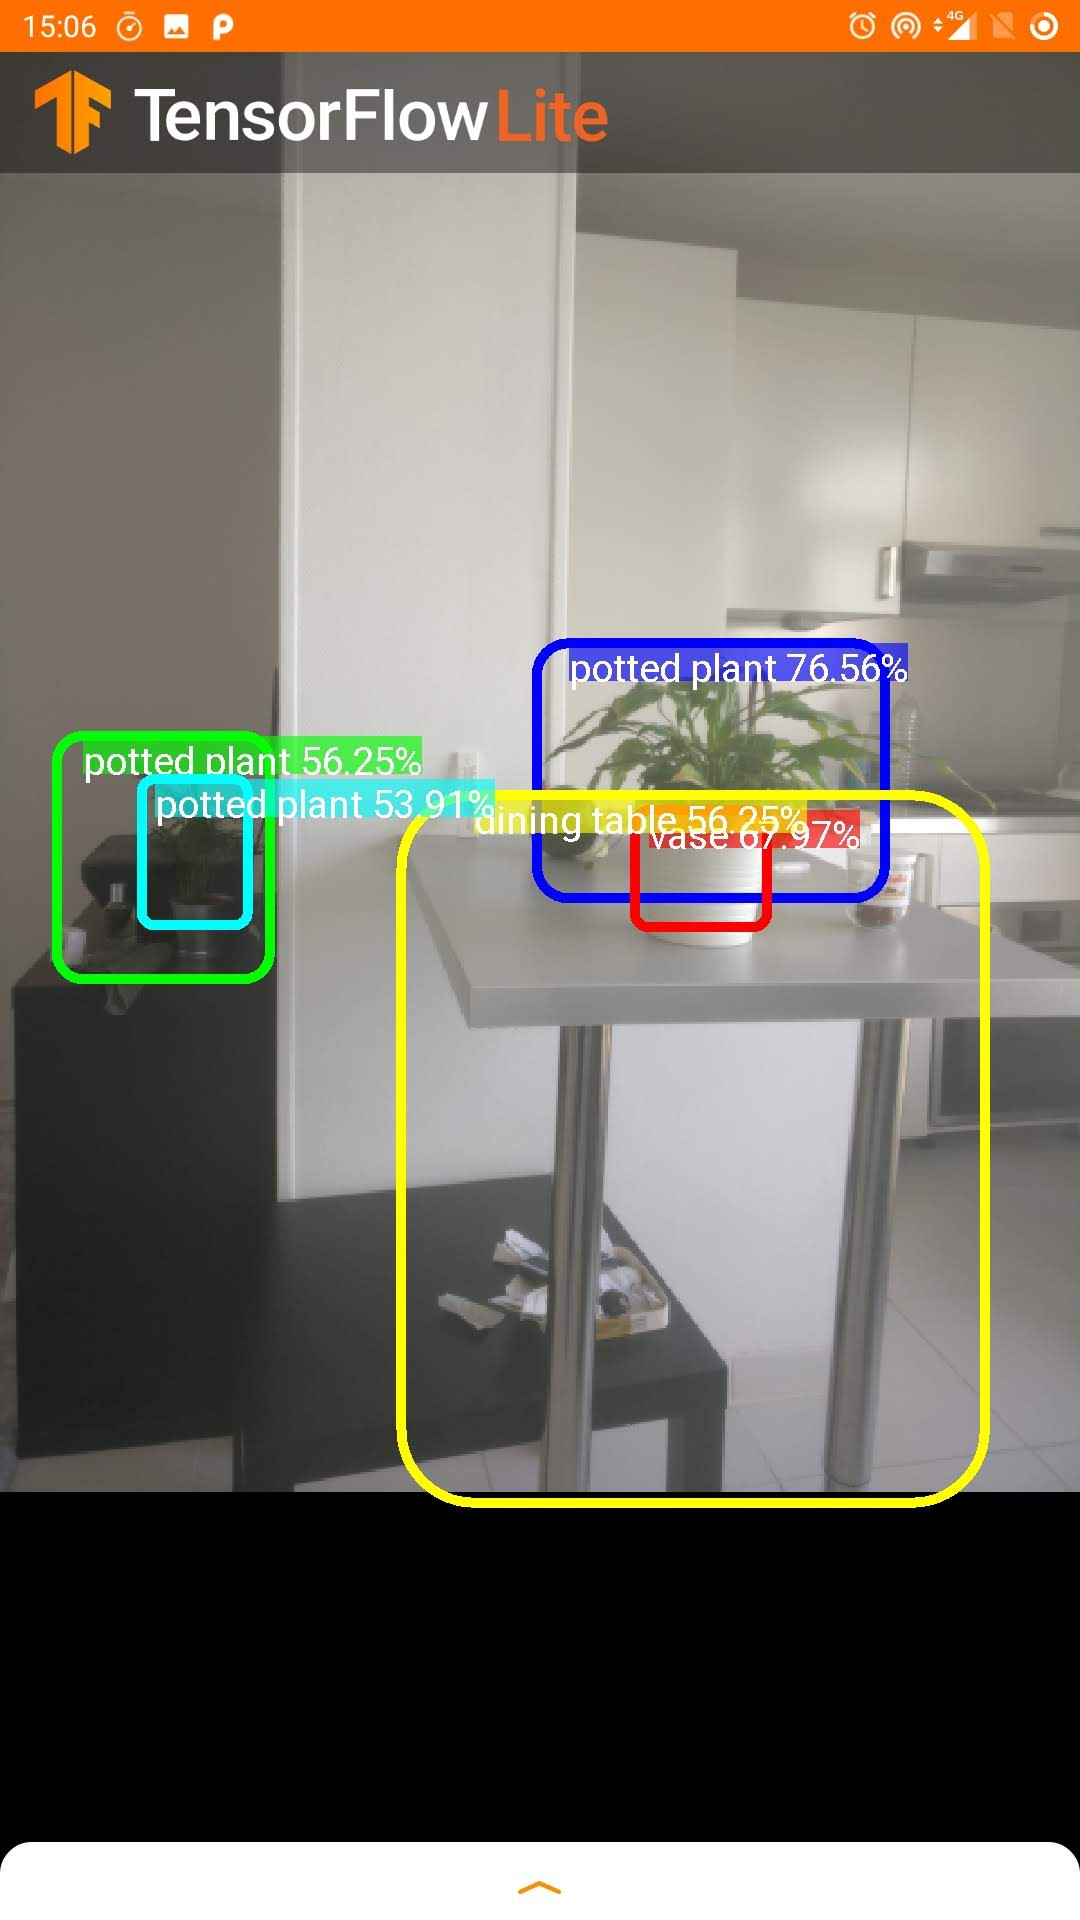
\includegraphics[width=0.3\textwidth]{images/multiobj.jpg}
  \caption{Ensemble des résultats retournés par le détecteur}
  \label{fig:multiobj}
\end{figure}

Il existe des modèles tels que les modèles de classification d'objet qui ne renvoie que le nom d'un seul élément sur une image (voir cahier d'analyse). Ce type de modèle, bien que plus précis, nous intéresse moins puisqu'on souhaite récupérer le maximum d'information sur la scène qui entoure l'utilisateur. Le fait d'utiliser un modèle qui nous renvoie le nom de chaque objet connu sur une image est donc une solution plus adaptée pour notre besoin. Cependant, cela crée un problème lorsqu'on souhaite informer l'utilisateur de tous ces objets détectés en utilisant le synthétiseur vocal. En effet, la liste des résultats retournés par le détecteur peut facilement être affiché visuellement avec le label et la position de l'objet de manière instantanée (comme sur la figure \ref{fig:multiobj}). Mais avec le synthétiseur vocal, impossible de citer chaque objet en continue de manière fluide et en temps réel selon l'image qu'il y a sur la scène. \\

Pour remédier à cela, on a réfléchi à un système de viseur virtuel. À l'image de l'oeil humain, ce viseur se chargera de se concentrer sur un point particulier de l'image (dans notre cas, le centre). Ensuite, ce sera l'objet visé par ce point centrale qui sera énoncé à l'aide du synthétiseur vocal. Comme l'oeil humain, les autres objets seront dans le champ de vision (autour du viseur), mais ne seront pas l'objet principal à citer. \\
\newpage

\begin{figure}[h!]
\centering
  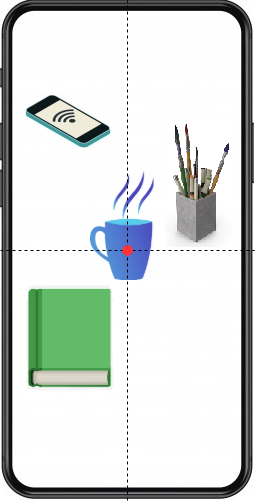
\includegraphics[width=0.3\textwidth]{images/viseur.png}
  \caption{Principe du viseur virtuel}
  \label{fig:viseur}
\end{figure}

Pour les autres objets, ces informations ne sont pas perdus. On garde précieusement ces informations qu'on pourra utiliser d'une autre manière (exemple: vibrer en fonction du nombre d'objet qu'il y a dans le champ de vision, ou rester appuyé pour que le synthétiseur nous indique chaque objet autour du viseur, etc.). Cela évite simplement d'encombrer le synthétiseur et de devenir agaçant pour l'utilisateur.\\

On rajoute ensuite dans le code une condition en plus avant d'énoncé un objet en vérifiant si l'objet est visé ou pas.\\

\begin{lstlisting}[language=Java]
for (Detector.Recognition r :results) {
  // ...
  if(r.getLocation().contains(viseurReco.getLocation())){ // Si le viseur est dans l'objet detecte
    if(!tts.isSpeaking() && !readedText.equals(r.getTitle())){
      tts.speak(r.getTitle(), TextToSpeech.QUEUE_FLUSH, null, null);
      readedText = r.getTitle();
    }
  }
  // ...
}
\end{lstlisting}

\newpage
Dans l'image ci-dessous, on a donc que le cahier qui est énoncé.\\

\begin{figure}[h!]
\centering
  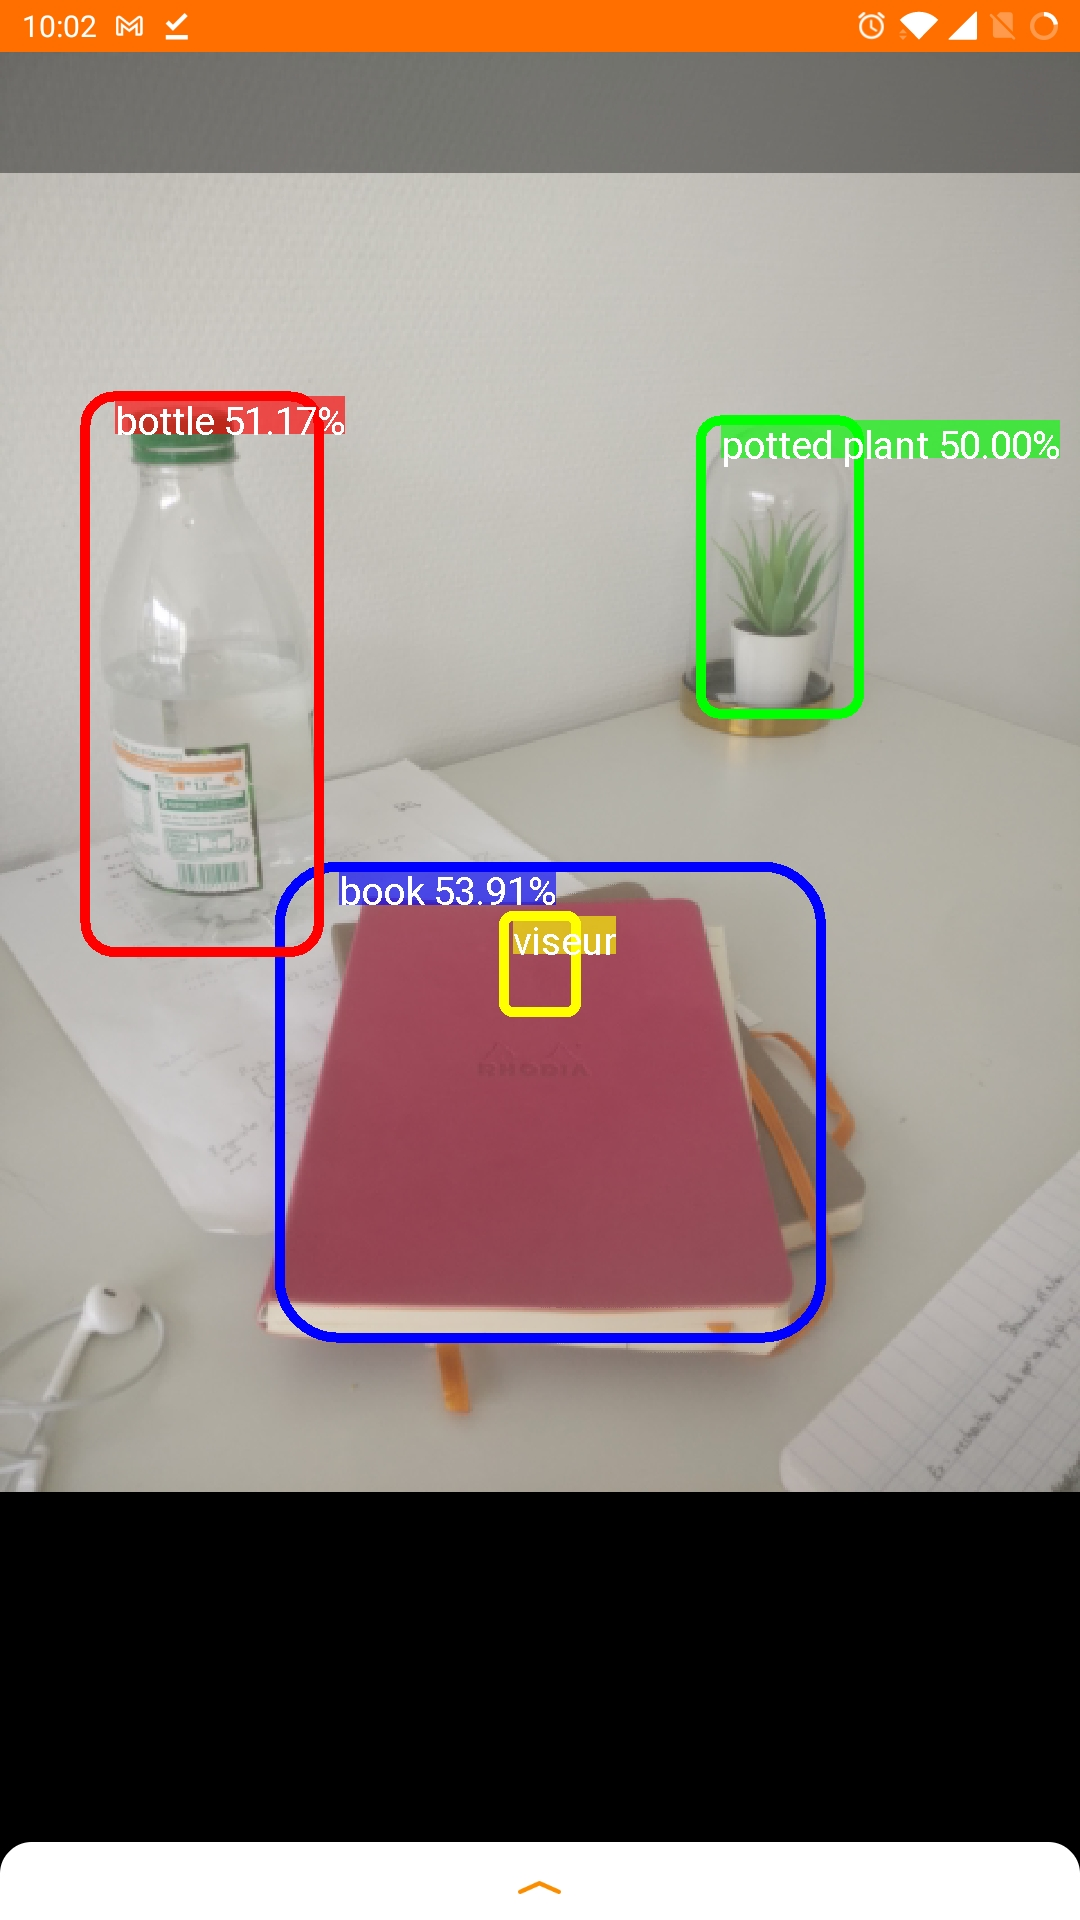
\includegraphics[width=0.3\textwidth]{images/viseurapp.jpg}
  \caption[]{Résultat du viseur \footnotemark}
  \label{fig:viseurapp}
\end{figure}

\footnotetext{Le viseur est affiché à titre indicatif mais son affichage n'est pas utile}

\section{Réglage du seuil de détection}

Pour réduire la multitude des objets détectés, j'ai ajouté la possibilité de modifier le seuil de détection minimale. En mettant un seuil plus élevé, on a moins d'objets détectés, mais ceux détectés sont donc moins sujet à l'erreur. On viendra donc placer une nouvelle condition pour trier les objets parmi ceux retournés en prenant uniquement celles qui ont un seuil au-dessus du seuil fixé :\\

\begin{lstlisting}[language=Java]
for (Detector.Recognition r :results) {
  // ...
  if(r.getConfidence() >= finalMinimumConfidence){
  	if(r.getLocation().contains(viseurReco.getLocation())){ // Si le viseur est dans l'objet detecte
	    if(!tts.isSpeaking() && !readedText.equals(r.getTitle())){
	      tts.speak(r.getTitle(), TextToSpeech.QUEUE_FLUSH, null, null);
	      readedText = r.getTitle();
	    }
    }
  }
  // ...
}
\end{lstlisting}

J'ai décidé de rajouter le réglage du seuil dans le volet inférieur car l'utilisateur n'aura probablement pas besoin de modifier ce paramètre. Le seuil par défaut est à 60\%.\\

\begin{figure}[h!]
\centering
  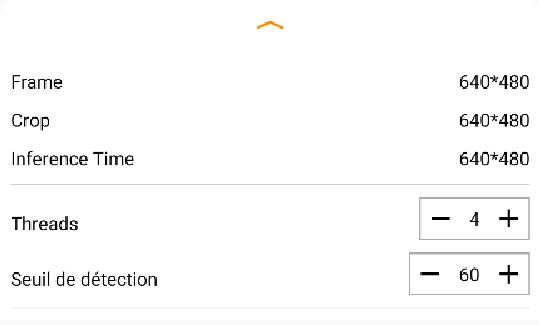
\includegraphics[width=0.3\textwidth]{images/seuil.JPG}
  \caption{Réglage du seuil de détection}
  \label{fig:seuil}
\end{figure}

En outre, si l'utilisateur souhaite modifier ce paramètre, il faudra ouvrir le volet en le glissant puis naviguer sur chaque élément avec le synthétiseur vocal par défaut de son smartphone (le mode voice assistant) \footnote{Remarque : L'activation du mode Voice Assistant n'interfère pas avec la synthèse vocal implémenté au sein de l'application. Il est donc possible d'utiliser ce mode par-dessus d'autres applications utilisant la synthèse vocal.}.

\section{Capteurs}

Toujours dans l'optique de découvrir les possibilités que peuvent nous apporter un smartphone, nous avons voulu tester l'utilisation de différents capteurs présents dans le téléphone. J'ai donc mis en place trois capteurs : \\

\begin{itemize}
  \item Le GPS
  \item Le gyroscope
  \item Le capteur de roation geomagnetique
  \item Le capteur de proximité \\
\end{itemize}

Sur Android pour utiliser ces capteurs, il suffit d'avoir un \verb|SensorManager| et une instance de chaque capteurs avec la classe \verb|Sensor|. Une fois les demandes de permissions ajouté si nécessaire dans le fichier Android Manifest, il suffit d'enregistrer chaque capteur avec un listener pour motirer leurs changement : \verb|registerListener(SensorEventListener listener, Sensor sensor,int samplingPeriodUs)|. À chaque changement, je vérifie ensuite le type du capteur et affiche la valeur renvoyé : \\

\begin{lstlisting}[language=Java]
public void onSensorChanged(SensorEvent event) {
    if(event.sensor.getType() == Sensor.TYPE_ROTATION_VECTOR){
      gyroscopeTV.setText("gyroscope: x="+event.values[0]+" y="+event.values[1]+" z="+event.values[2]);
      gyroscopeTV.setTextColor(Color.WHITE);
    }
    if(event.sensor.getType() == Sensor.TYPE_PROXIMITY){
      proximityTV.setText("proximite: "+event.values[0]+" cm");
      proximityTV.setTextColor(Color.WHITE);
    }
    if (event.sensor.getType() == Sensor.TYPE_GEOMAGNETIC_ROTATION_VECTOR){
      geomagneticTV.setText("geomagnetique: x="+event.values[0]+" y="+event.values[1]+" z="+event.values[2]);
      geomagneticTV.setTextColor(Color.WHITE);
    }
  }
\end{lstlisting}

En utilisant le GPS, on peut reproduire les fonctionnalités que proposent les cannes connectées aujourd'hui comme la géolocalisation de l'utilisateur. Cette géolocalisation peut être utilisée pour informer les proches du lieu où se trouve l'utilisateur en cas de danger, mais il peut aussi servir à enregistrer des informations sur un lieu spécifique. En effet, à l'aide des autres capteurs, il pourra être envisagé la création d'une cartographie en se basant sur le lieu et l'orientation en fonction des pôles (Nord, Sud, Est, Ouest). Ainsi, l'ensemble des objets détectés sur une image pourra être enregistré et attribuer à un emplacement spécifique dans l'espace. Cela permettra de guider par exemple l'utilisateur sur un lieu où il a l'habitude de se rendre régulièrement.

\section{Documentations}

\begin{figure}[h!]
\centering
  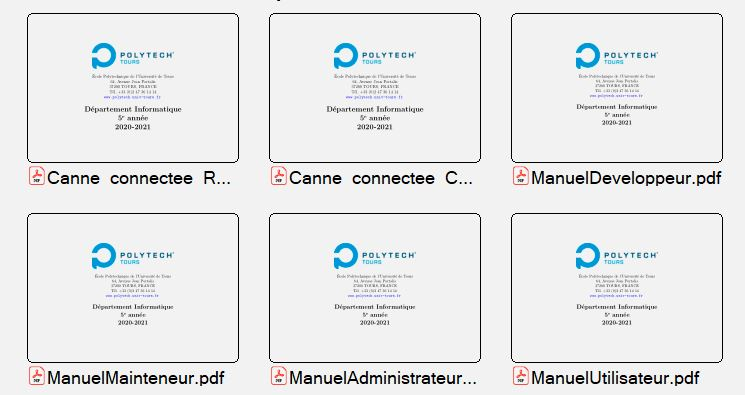
\includegraphics[width=\textwidth]{images/docs.JPG}
  \caption{Documentations}
  \label{fig:docs}
\end{figure}

Ce rapport n'étant qu'une synthèse du travail réalisé, il est accompagné de divers document permettant d'avoir plus de détails sur différents points du projet. Pour que mon travail puisse être repris facilement, j'ai pris soin de fournir un maximum d'informations pour répondre aux éventuelles interrogations. Ces ressources permettront donc à d'autres étudiants d'utiliser le travail réalisé afin de travailler sur la canne connectée.

\section{Résultat final}

Ce projet a permis d'aboutir sur une application Android stable renvoyant des données utiles au sein d'un environnement donnée. L'application est capable de renvoyer sous forme audio les objets détectés afin que cela puisse être utilisé par les personnes malvoyantes. 

\begin{figure}[h!]
\centering
  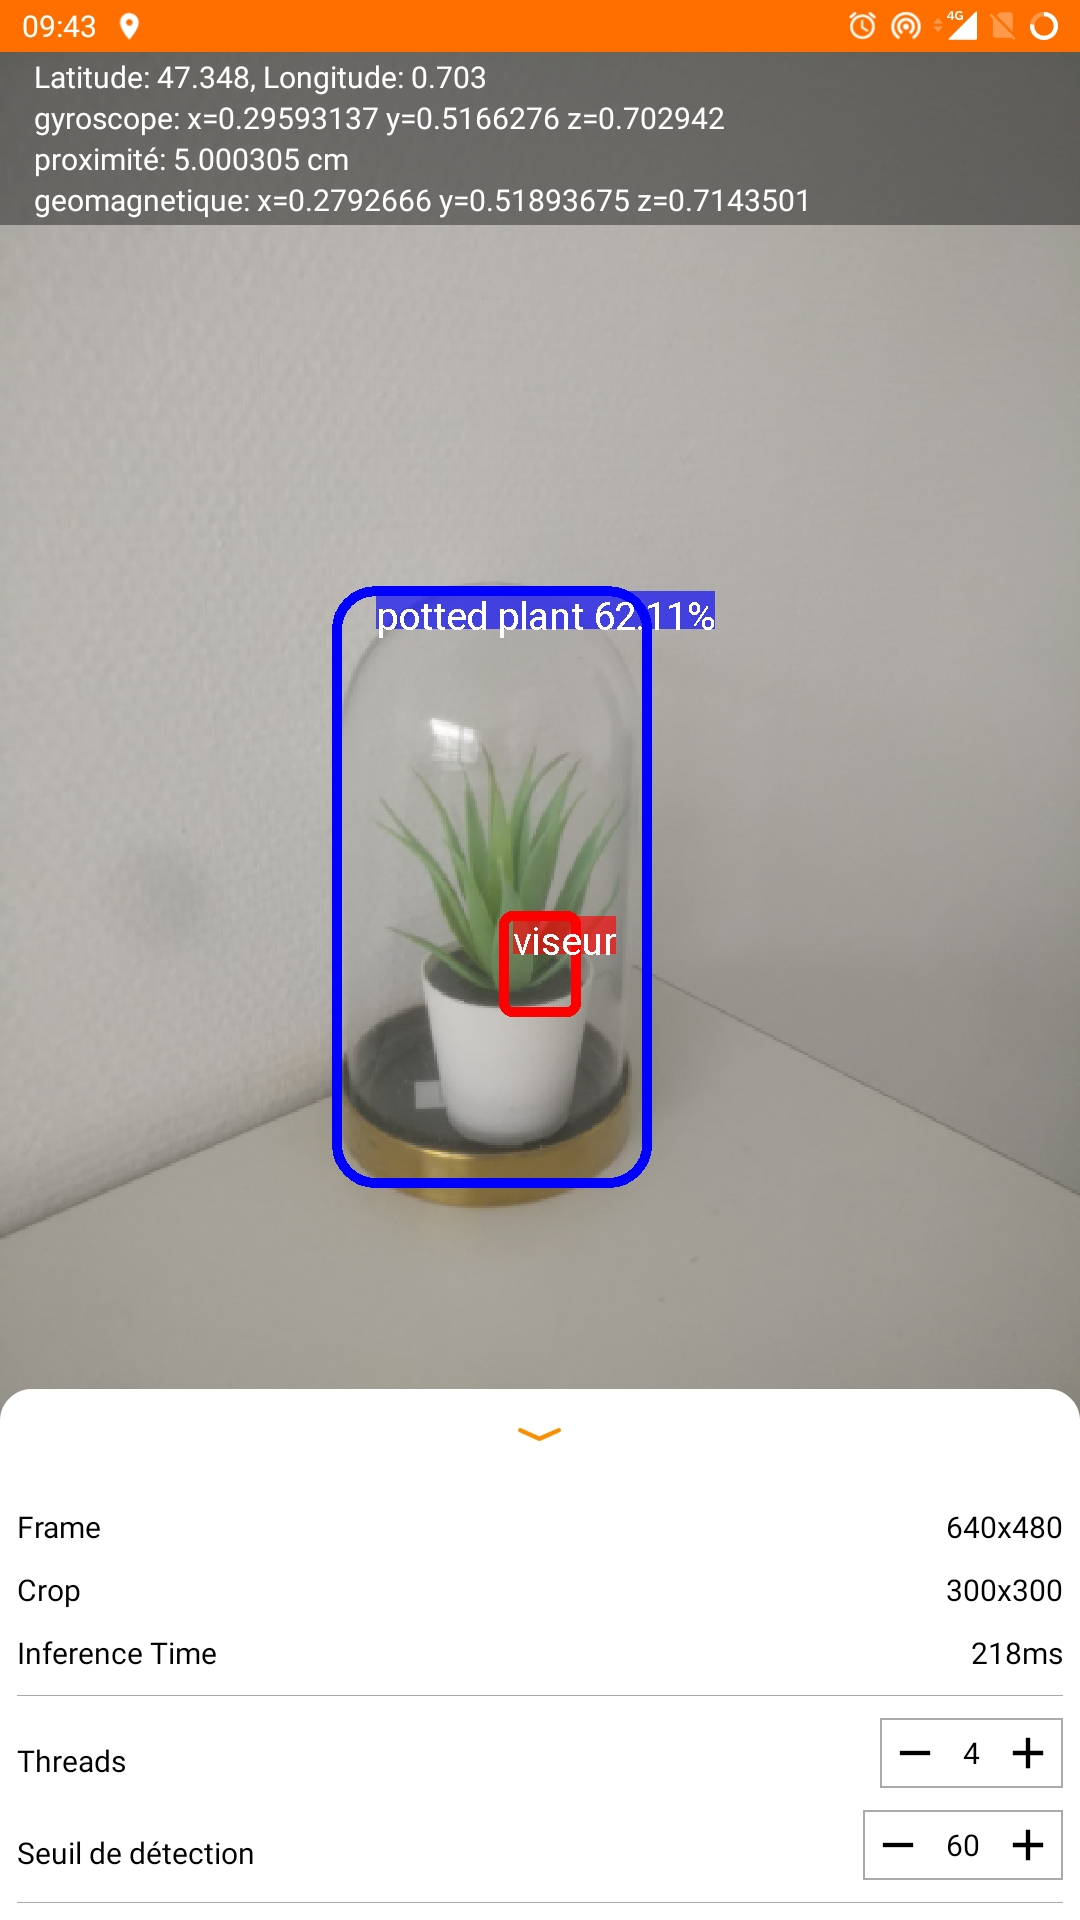
\includegraphics[width=0.3\textwidth]{images/result.jpg}
  \caption{Résultat final}
  \label{fig:result}
\end{figure}

Les données renvoyées par les capteurs (localisation, orientation, etc.) restent cependant à utiliser à travers des fonctionnalités qui pourront être utiles aux aveugles. Le projet peut donc être présenté à des aveugles afin d'avoir un premier retour sur les fonctionnalités qu'ils souhaiteraient retrouver au sein de ce type d'application.

\chapter{Prise de recul}

\section{Points positifs}

Du point de vue de l'application, je suis assez satisfait de ce qui a été réalisé. En effet, l'application répond au besoin initial qui a été défini en début de projet. Les fonctionnalités de base ont été implémentés tel que la détection d'objet et le retour vocal. Egalement, j'ai réussi à explorer certaines possibilités que peuvent apporter le smartphone notamment en utilisant les différents capteurs qui y sont intégrés. J'ai également pu souligner une limite sur la partie détection d'objet qui est l'emboitement des objets détectés. Avec cette limite, on prend donc conscience que l'intelligence artificielle atteint aujourd'hui des résultats très satisfaisant mais présente encore quelques problèmes lorsqu'on souhaite le mettre à profit sur des cas concrèt.\\

D'un point de vue gestion de projet, j'ai su allier travail et communication réguliere avec le client. Le travail réalisé a pu suivre un planning bien établi à l'avance afin d'anticiper les délais et jalons prévu par Polytech. Les communications régulieres avec le client ont permis de faire un point sur l'avancé du projet de manière hebdomadaire. galement l'effort dans la mise en place d'un Git ainsi que la rédaction des divers documents pourra permettre une réutilisabilité de mon travail.\\

Dans l'ensemble, j'ai apprécié travaillé sur ce projet avec M.VENTURINI qui a su me guider tout au long de ce projet. J'ai pu mettre en pratique mes connaissances et en apprendre davantage concernant l'intelligence artificielle.

\section{Points critiques}

Malgré les résultats obtenus, l'application est exploitable, mais plusieurs fonctionnalités peuvent encore être implémentés. En effet, toutes les possibilités du smartphone n'ont pas pu être mis en oeuvre faute de temps. On aurait pu en effet, comme l'a suggéré M.VENTURINI, implémenté en plus de la détection d'objet, un système de navigation se basant sur une cartographie alimentée par les objets détectés sur un lieu donné. Ainsi on met en oeuvre la géolocalisation, l'orientation du smartphone, et bien d'autres capteurs qui sont présents sur le smartphone. Le PFE ne durant qu'à peine cinq mois, et tenant compte des obligations scolaires en parallèle, ce point a été une des plus critiques.\\

En terme de gestion de projet, le projet ne m'a pas permis de faire une gestion budgétaire par exemple puisque je n'ai eu aucune commande de matériel à faire à la comptabilité de l'école. L'école disposant déjà de smartphone dédié pour les TPs. Le projet ne nécessite que ce matériel pour pouvoir être réalisé. Cela aurait pu être intéressant de pouvoir anticiper les coûts de différents matériels par exemple et de gérer le montant d'une commande afin que cela ne dépasse pas le budget du projet. Puiqu'un projet tourne autour des trois points : coût, délai et qualité, je n'ai pas eu l'occasion de gérer la partie coût. Pour estimer le coût du projet, j'ai utilisé un Samsung Galaxy S10e 128Go de l'école qui coûte 449€. À cela s'ajoute le temps de travail d'un apprenti ingénieur.

\section{Difficultés}

L'une des difficultés que j'ai rencontré lors de ce projet fut la montée en compétence dans le domaine de l'intelligence artificielle. En effet, durant toute ma scolarité je n'ai pas eu l'occasion de suivre des cours sur ce thème afin d'avoir quelques bases sur son fonctionnement. J'ai donc du chercher à comprendre rapidement les éléments dont j'aurai besoin pour ce projet sans forcément m'attarder sur le fonctionnement interne des réseaux de neurones. En effet, durant mes recherches afin de gagner du temps, je ne me suis pas plongé sur le fonctionnement en détail d'un réseau de neurone ainsi que des procédés mathématiques qui y sont employées. C'est le point que je trouve dommage puisque cela m'aurait permis d'en apprendre beaucoup mais dans le cadre de ce projet je n'ai pas eu besoin d'aller aussi loin. Il a donc fallu trier les informations et prendre que ce qui m'est utile pour la réalisation du projet. Mais dans l'ensemble j'ai quand même appris les grandes lignes et ça m'a permis de réaliser l'application.\\

Un autre point où j'ai eu assez de difficultés fut dans la rédaction des différents documents demandés. J'ai du accorder autant de temps à la rédaction de ce document qu'au développement de l'application. Le projet cette année étant axé sur ce point entre autre, je trouve que cela a quand même impacté grandement le travail réalisé concrètement au niveau de l'application.

\section{Améliorations possibles}

Parmi les améliorations que je pourrai faire ce serait dans la gestion du temps de travail accordé au projet. J'ai remarqué que travailler une ou deux heures par jour dans la semaine entre les cours était moins efficace que de bloquer toute une journée ou demi-journée sur le projet. En effet, j'ai trouvé qu'en une heure ou deux seulement, il m'est difficile d'être assez concentré et plongé dans le travail afin d'avancer considérablement.\\

Il y a plusieurs améliorations qui peuvent-être faites sur l'application. Parmi celles-ci :\\

\begin{itemize}
  \item Utiliser les données renvoyées par les capteurs pour d'autres fonctionnalités en plus (ex: situer le smartphone, détection de chutes, etc.)
  \item Sauvegarder les objets dans le champ de vision (objets non visés) dans une base de données pour constituer une cartographie des objets sur un lieu (ex: pièce de maison)
  \item Ajouter des fonctions de paramétrage avec des gestes sur l'écran (ex: régler le volume en glissant vers le haut/bas)\\
\end{itemize}

Ces suggestions d'améliorations sont bien sûr discutables en fonction de leurs utilités.

\chapter{Conclusion}

À travers ce projet, j'ai pu mettre en pratique mes connaissances et compétences apprises à Polytech Tours tout en apprenant de nouvelles. J'ai pu mettre en place une démarche ingénieur tout le long du projet à travers l'étude des besoins, la gestion du projet, la réalisation ainsi que la documentation. \\

Je suis content d'avoir pu livrer une version fonctionnelle et stable de l'application. Le respect des bonnes pratiques de programmation m'a permis d'avoir une application fluide et ainsi éviter d'avoir une application qui rame voir qui crash. Avec ce projet, j'espère avoir contribué à un travail qui sera utile aux personnes malvoyantes ou aveugles.\\

Ce fut un plaisir de travailler sur ce projet et d'apprendre beaucoup de notion sur l'intelligence artificielle. J'espère que j'aurai à nouveau une occasion pareille durant ma carrière pour renforcer et mettre en pratique ces connaissances.

\annexes

\end{document}